\graphicspath{{./images/molecules/orbitals/cis-pyrene/}}
\begin{figure}[h!]
	\centering
\begin{minipage}{\textwidth}\centering
\mybox{
\begin{tabular}{lrccc}
\multicolumn{2}{c}{\textbf{Cis-Pyrene}} & Model & HOMO & LUMO\\
\multicolumn{2}{c}{\textbf{}}
&\multirow{3}{*}{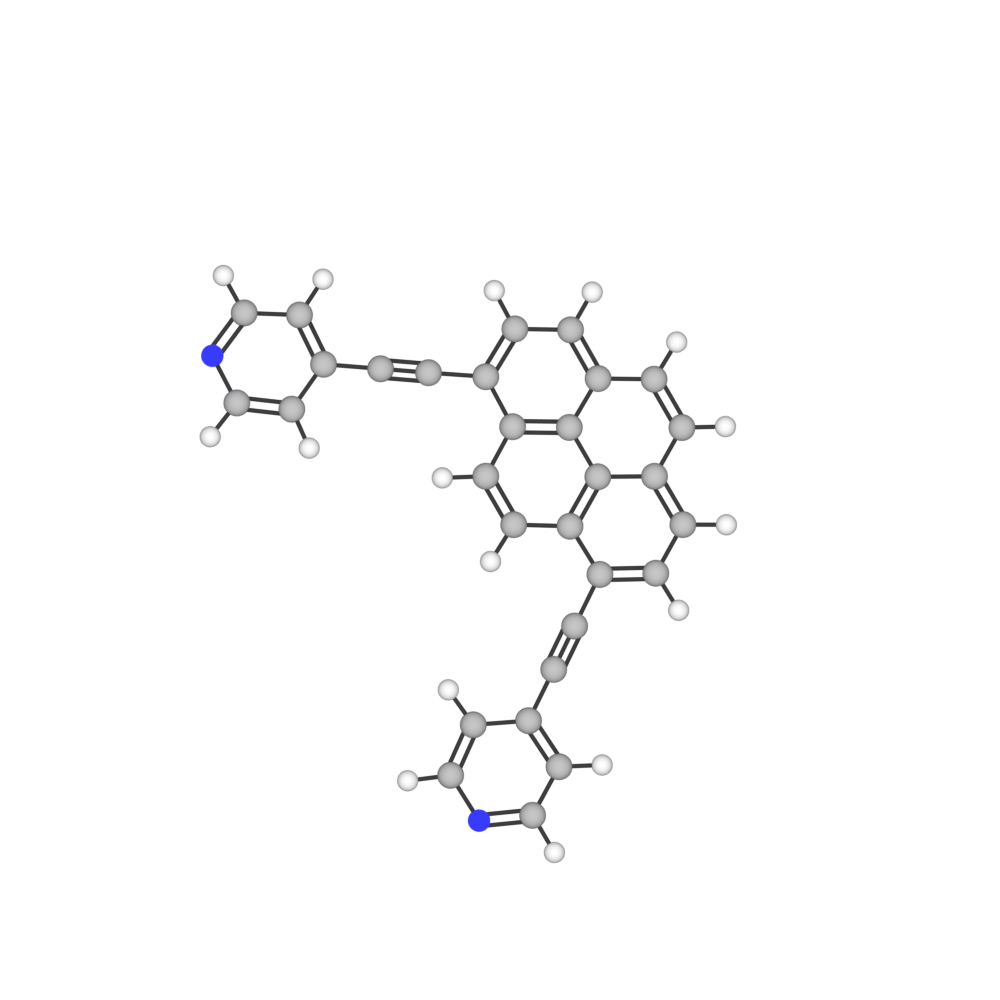
\includegraphics[width=2.7cm]{model}}
&\multirow{3}{*}{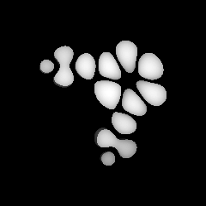
\includegraphics[width=2.7cm]{homo}}
&\multirow{3}{*}{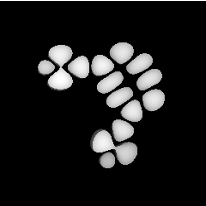
\includegraphics[width=2.7cm]{lumo}}\\
&&&& \\
\# Atoms & &&&\\
\# $e^-$ & 146 &&&\\
\# Orbitals & 85 &&&\\
$E_{Gap}$ &  \SI{}{\electronvolt} &&& \\
&&&& \\
&&& \SI{-11.601}{\electronvolt} & \SI{-10.134 }{\electronvolt} \\
\end{tabular}
}
\end{minipage}
	\subfigure[]{
		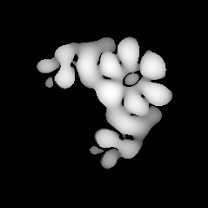
\includegraphics[width=2.7cm]{int-homo-1}
		\label{fig:}
	}
	\subfigure[HOMO - 1]{
		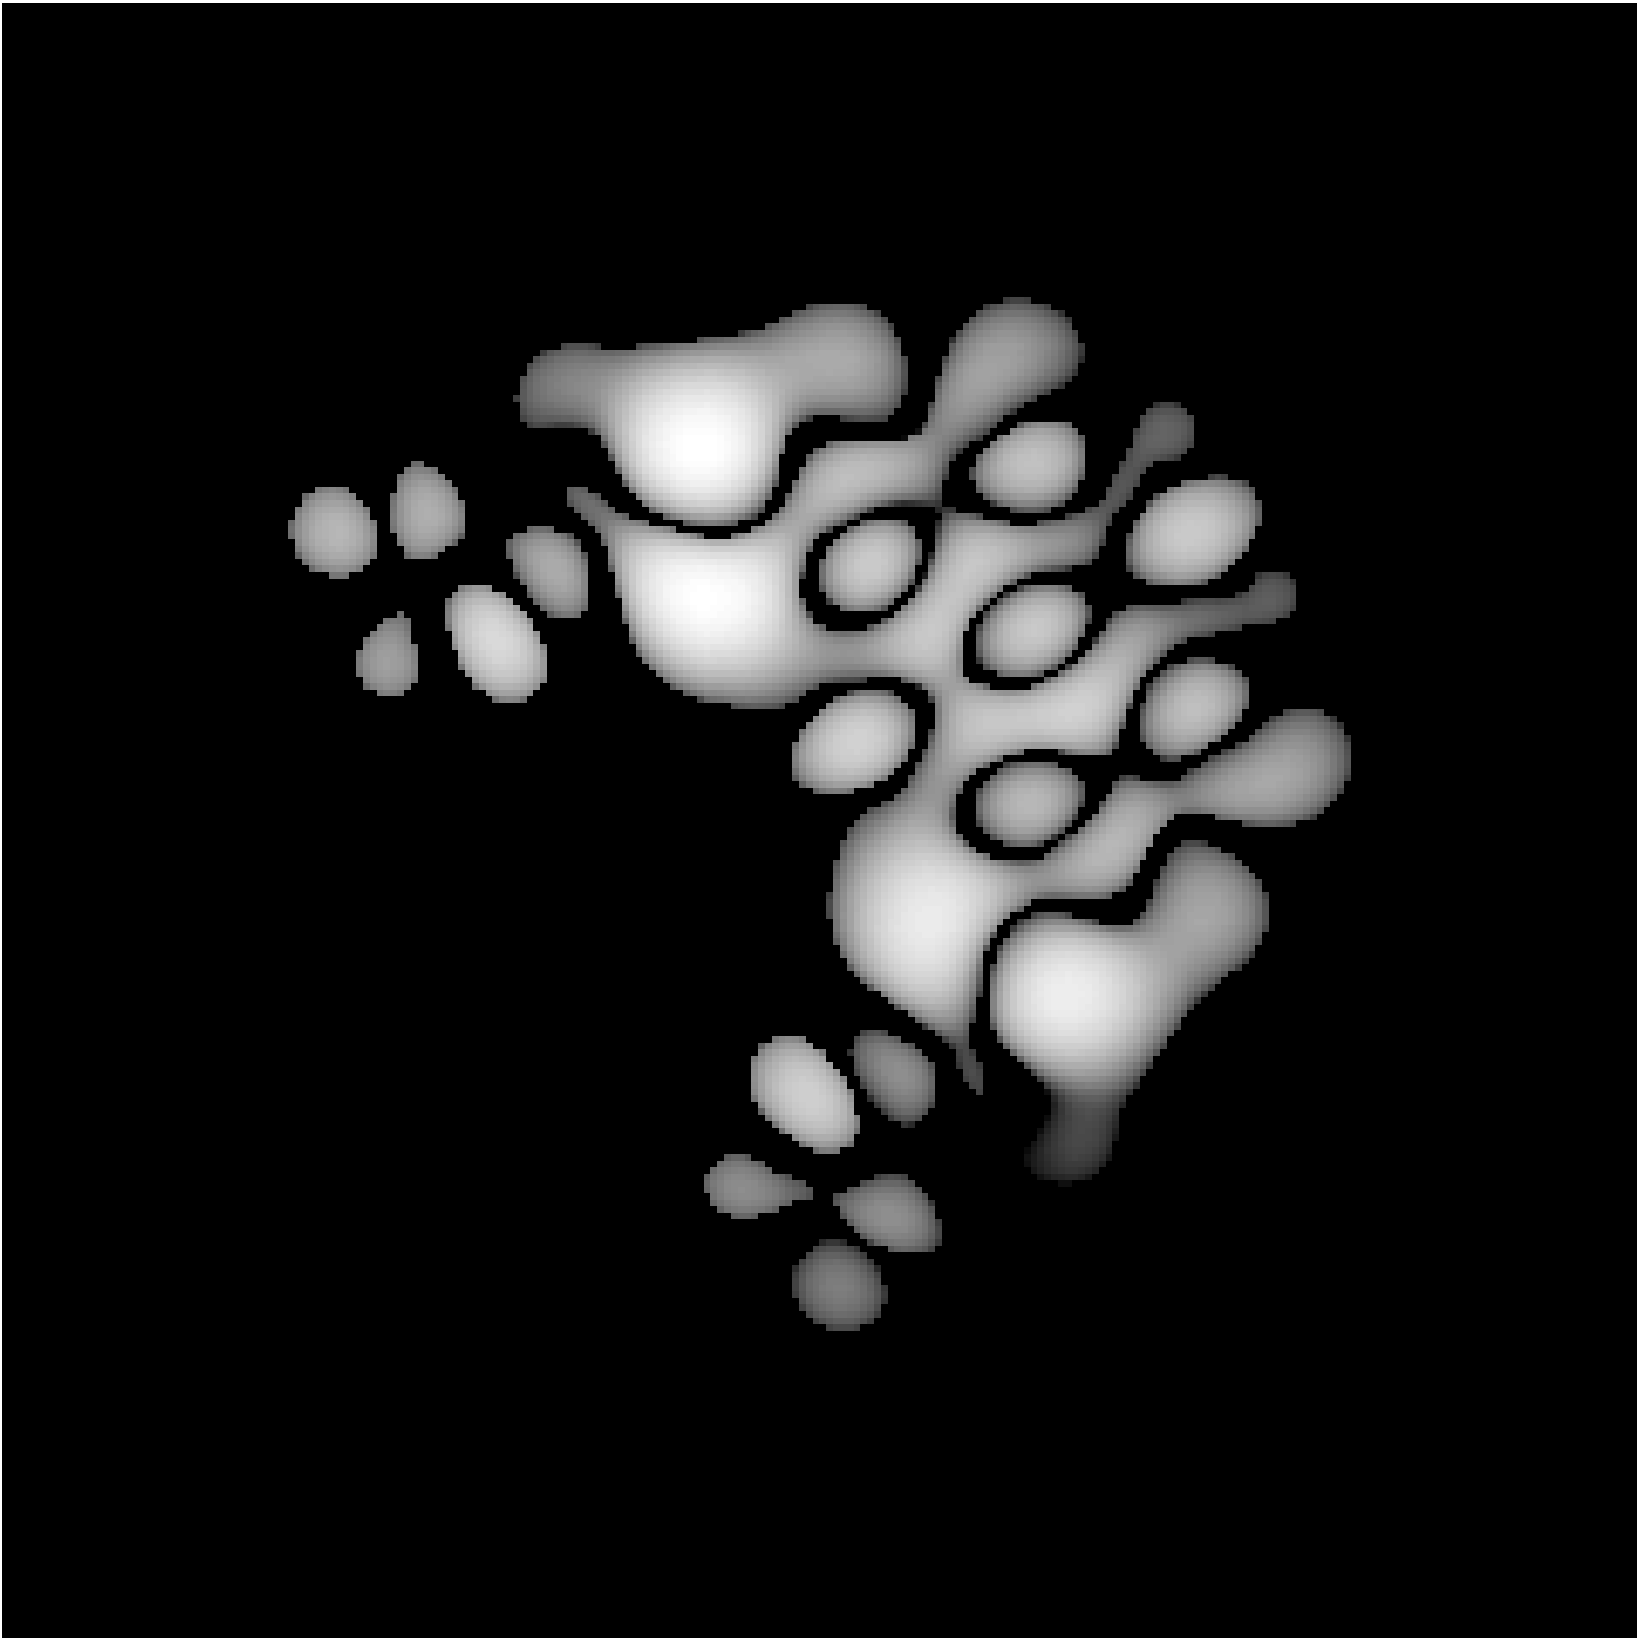
\includegraphics[width=2.7cm]{homo-1}
		\label{fig:homo-1}	
	}
	\subfigure[LUMO + 1]{
		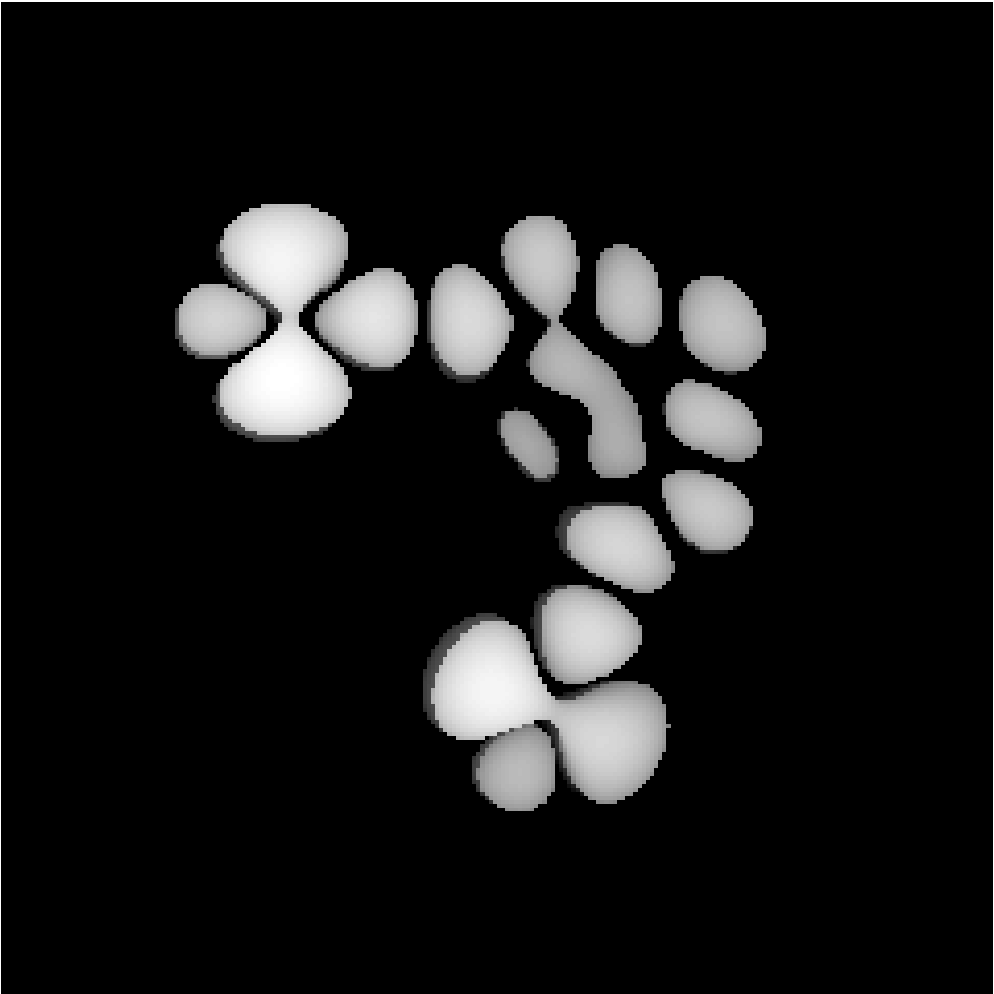
\includegraphics[width=2.7cm]{lumo-1}
		\label{fig:lumo+1}	
	}
	\subfigure[]{
		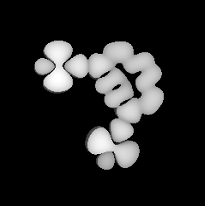
\includegraphics[width=2.7cm]{int-lumo-1}
		\label{fig:}	
	}
	%%%%%%%%%%%%%%%%%%%%%%%%%%%%%%%%%%%%%%%%%
	\subfigure[]{
		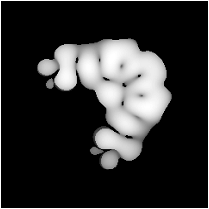
\includegraphics[width=2.7cm]{int-homo-2}
		\label{fig:}
	}
	\subfigure[HOMO - 2]{
		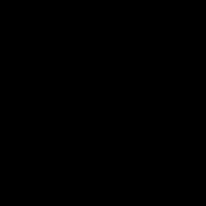
\includegraphics[width=2.7cm]{homo-2}
		\label{fig:homo-2}	
	}
	\subfigure[LUMO + 2]{
		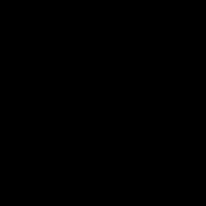
\includegraphics[width=2.7cm]{lumo-2}
		\label{fig:lumo+2}	
	}
	\subfigure[]{
		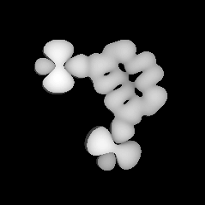
\includegraphics[width=2.7cm]{int-lumo-2}
		\label{fig:}	
	}
	%%%%%%%%%%%%%%%%%%%%%%%%%%%%%%%%%%%%%%%%%
	\subfigure[]{
		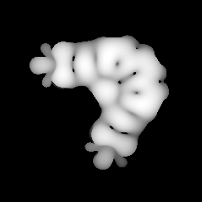
\includegraphics[width=2.7cm]{int-homo-3}
		\label{fig:}
	}
	\subfigure[HOMO - 3]{
		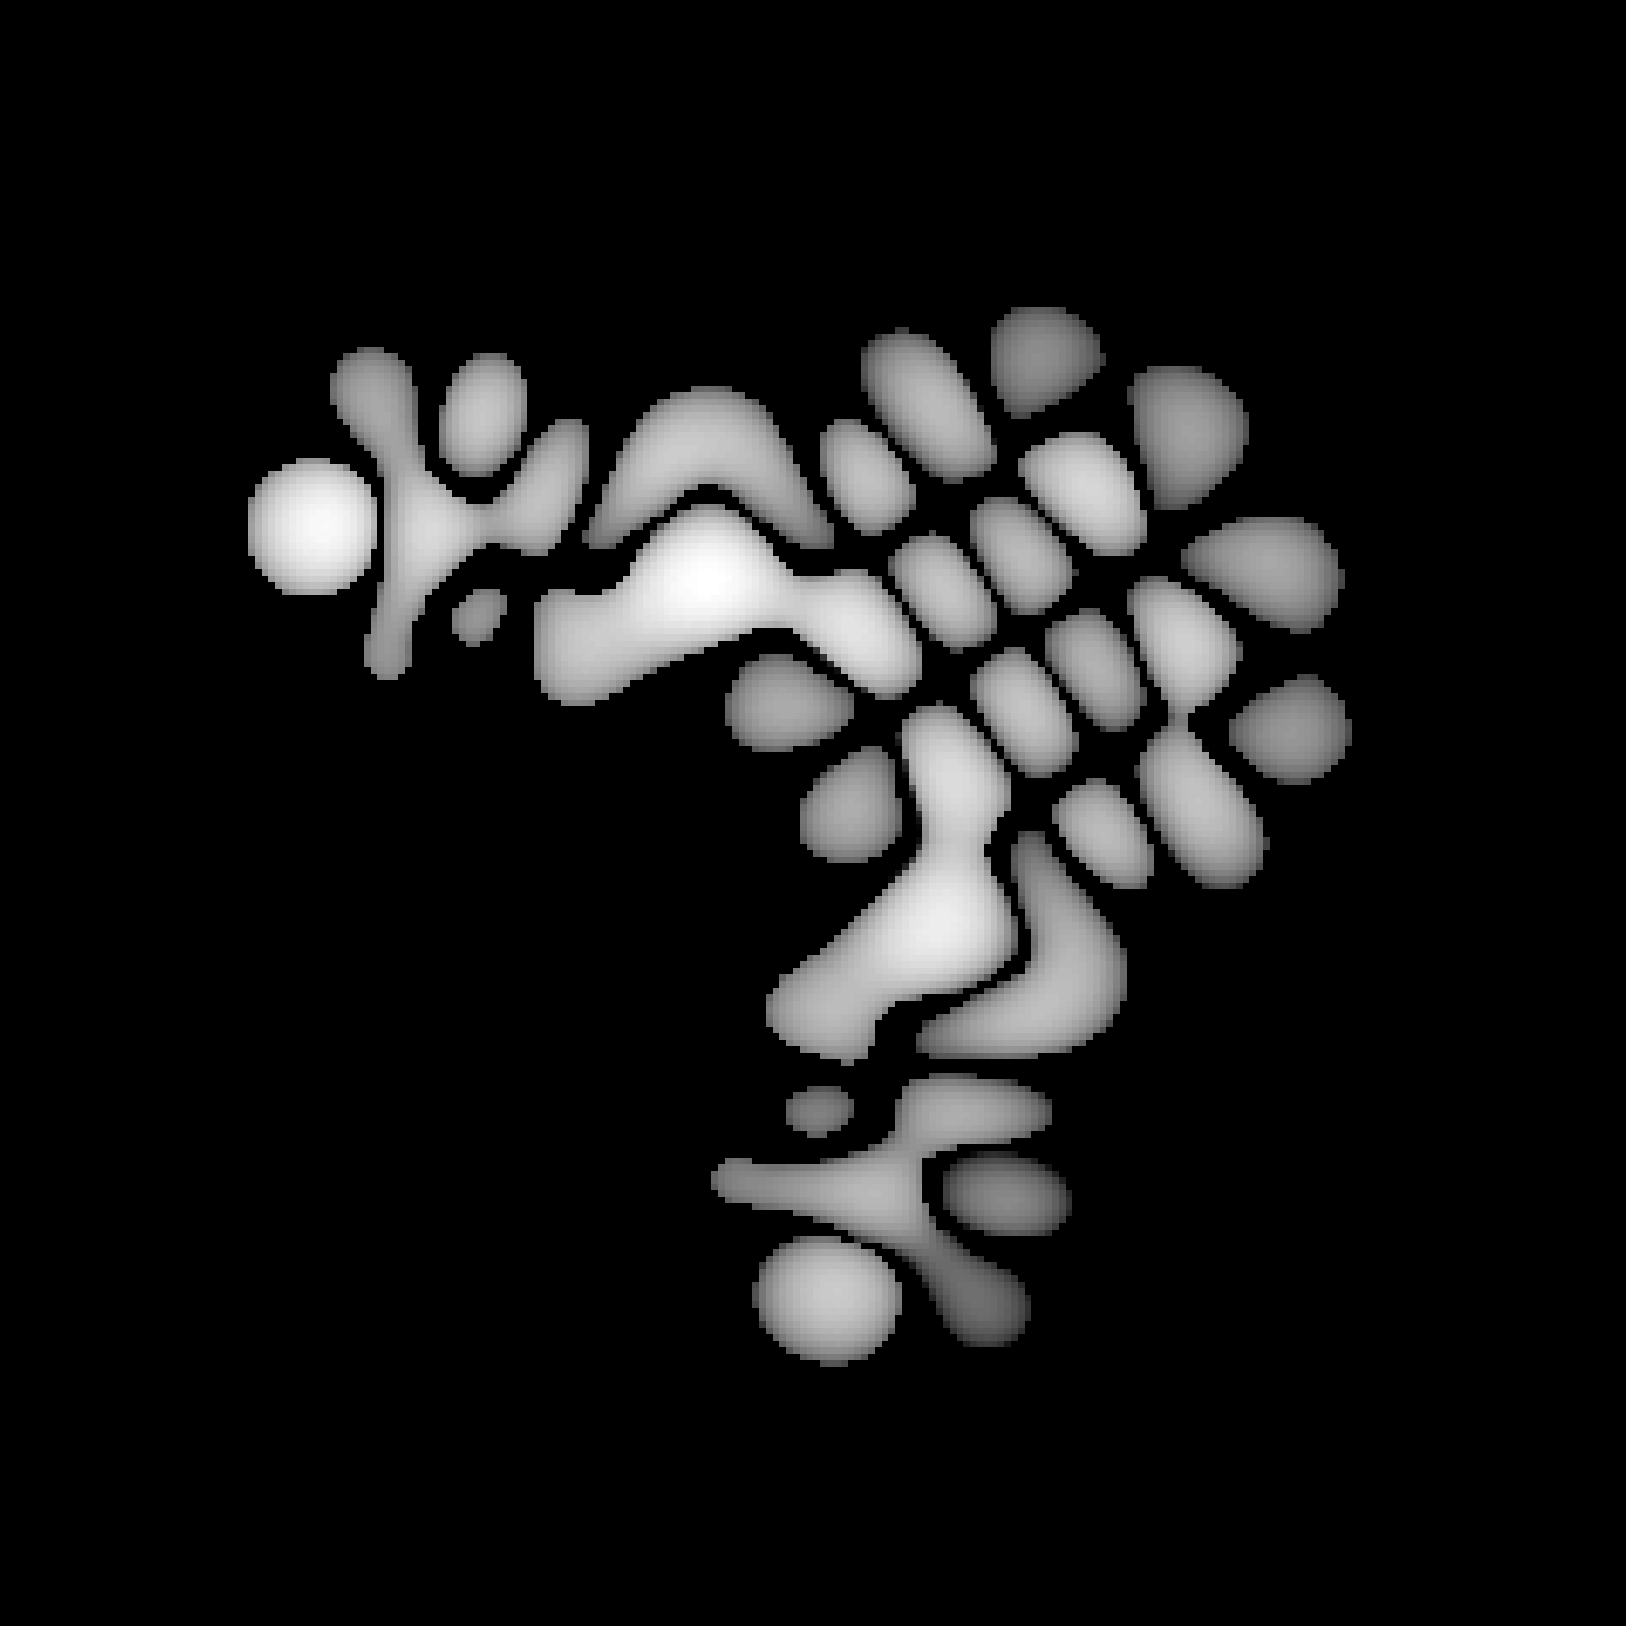
\includegraphics[width=2.7cm]{homo-3}
		\label{fig:homo-3}	
	}
	\subfigure[LUMO + 3]{
		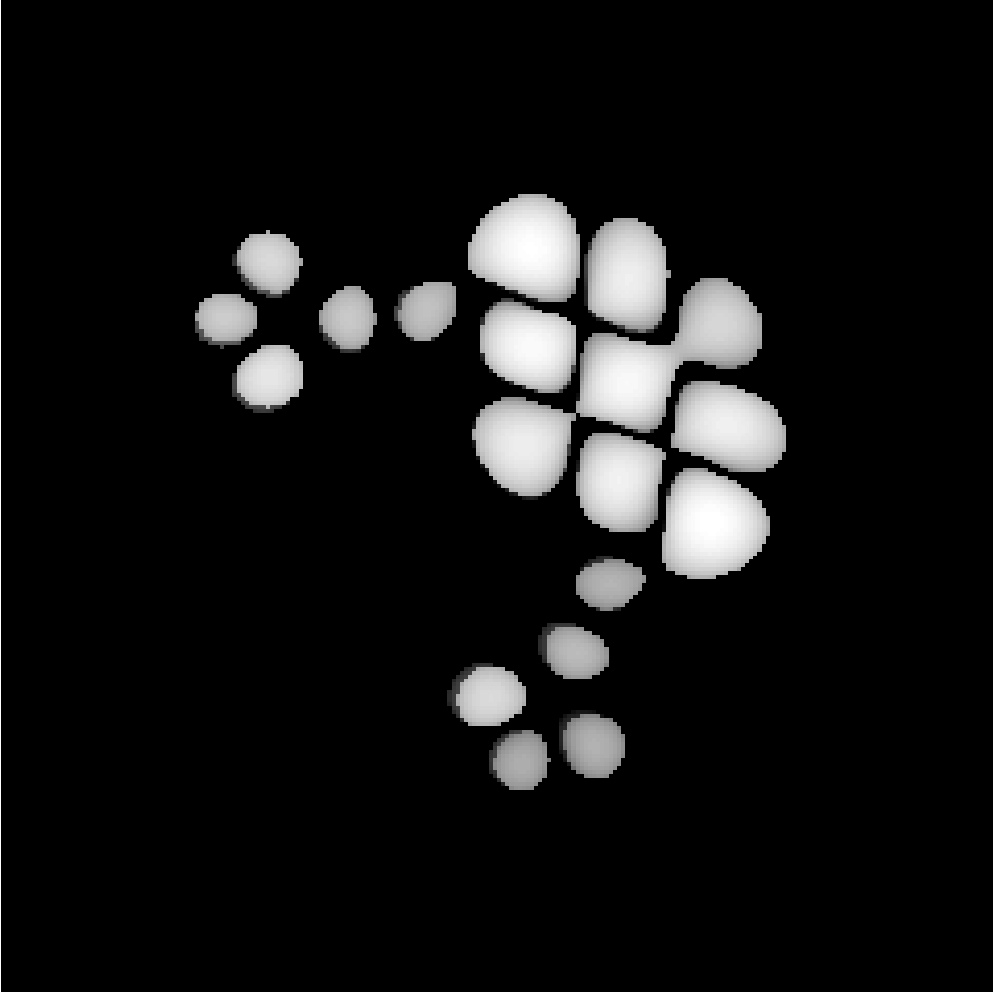
\includegraphics[width=2.7cm]{lumo-3}
		\label{fig:lumo+3}	
	}
	\subfigure[]{
		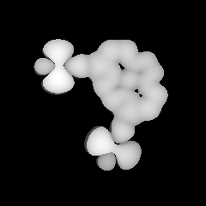
\includegraphics[width=2.7cm]{int-lumo-3}
		\label{fig:}	
	}
	%%%%%%%%%%%%%%%%%%%%%%%%%%%%%%%%%%%%%%%%%
	\subfigure[]{
		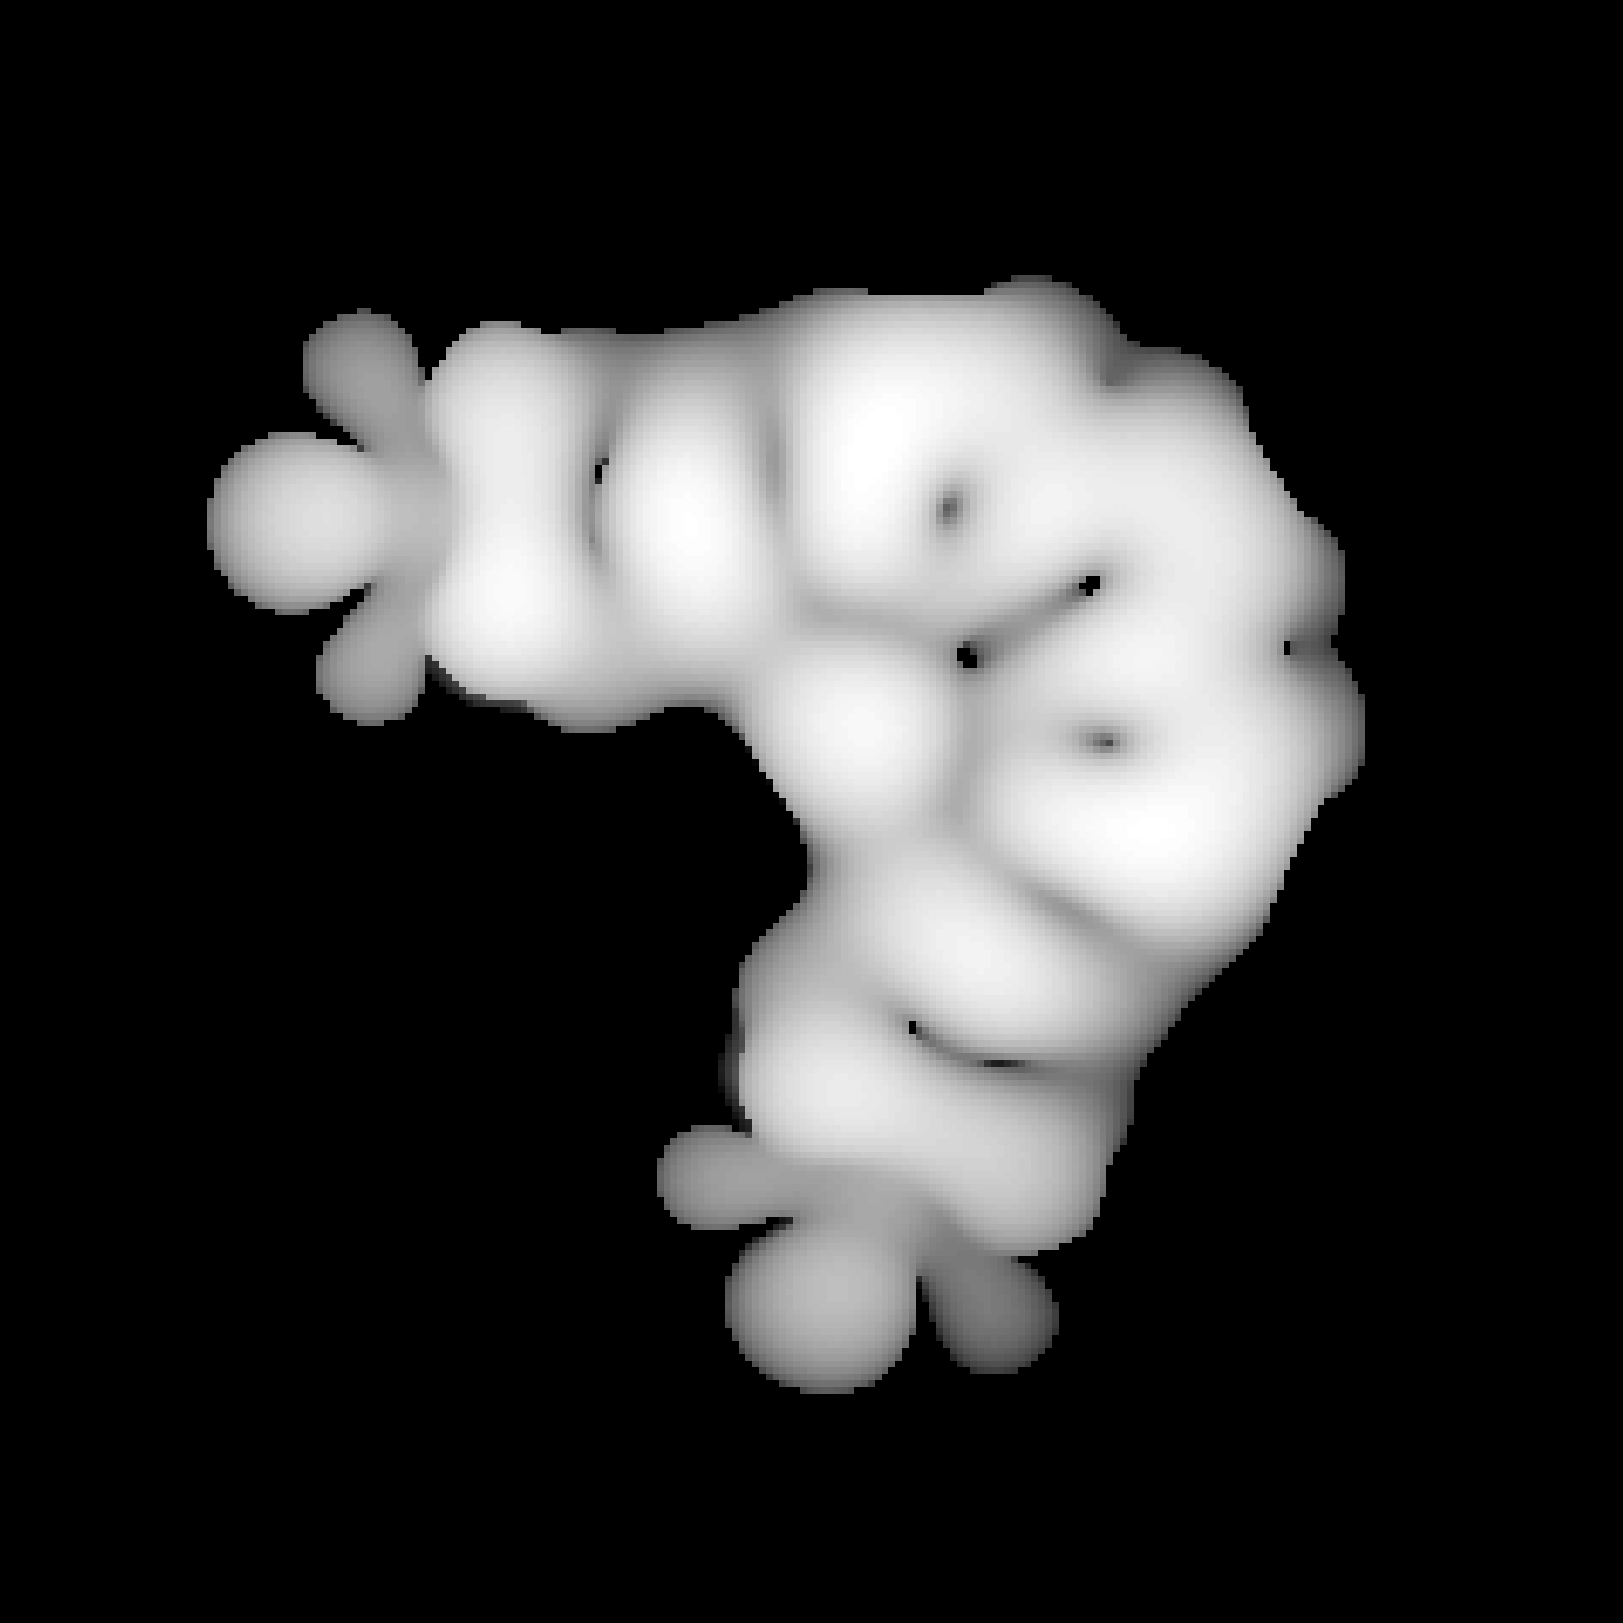
\includegraphics[width=2.7cm]{int-homo-4}
		\label{fig:}
	}
	\subfigure[HOMO - 4]{
		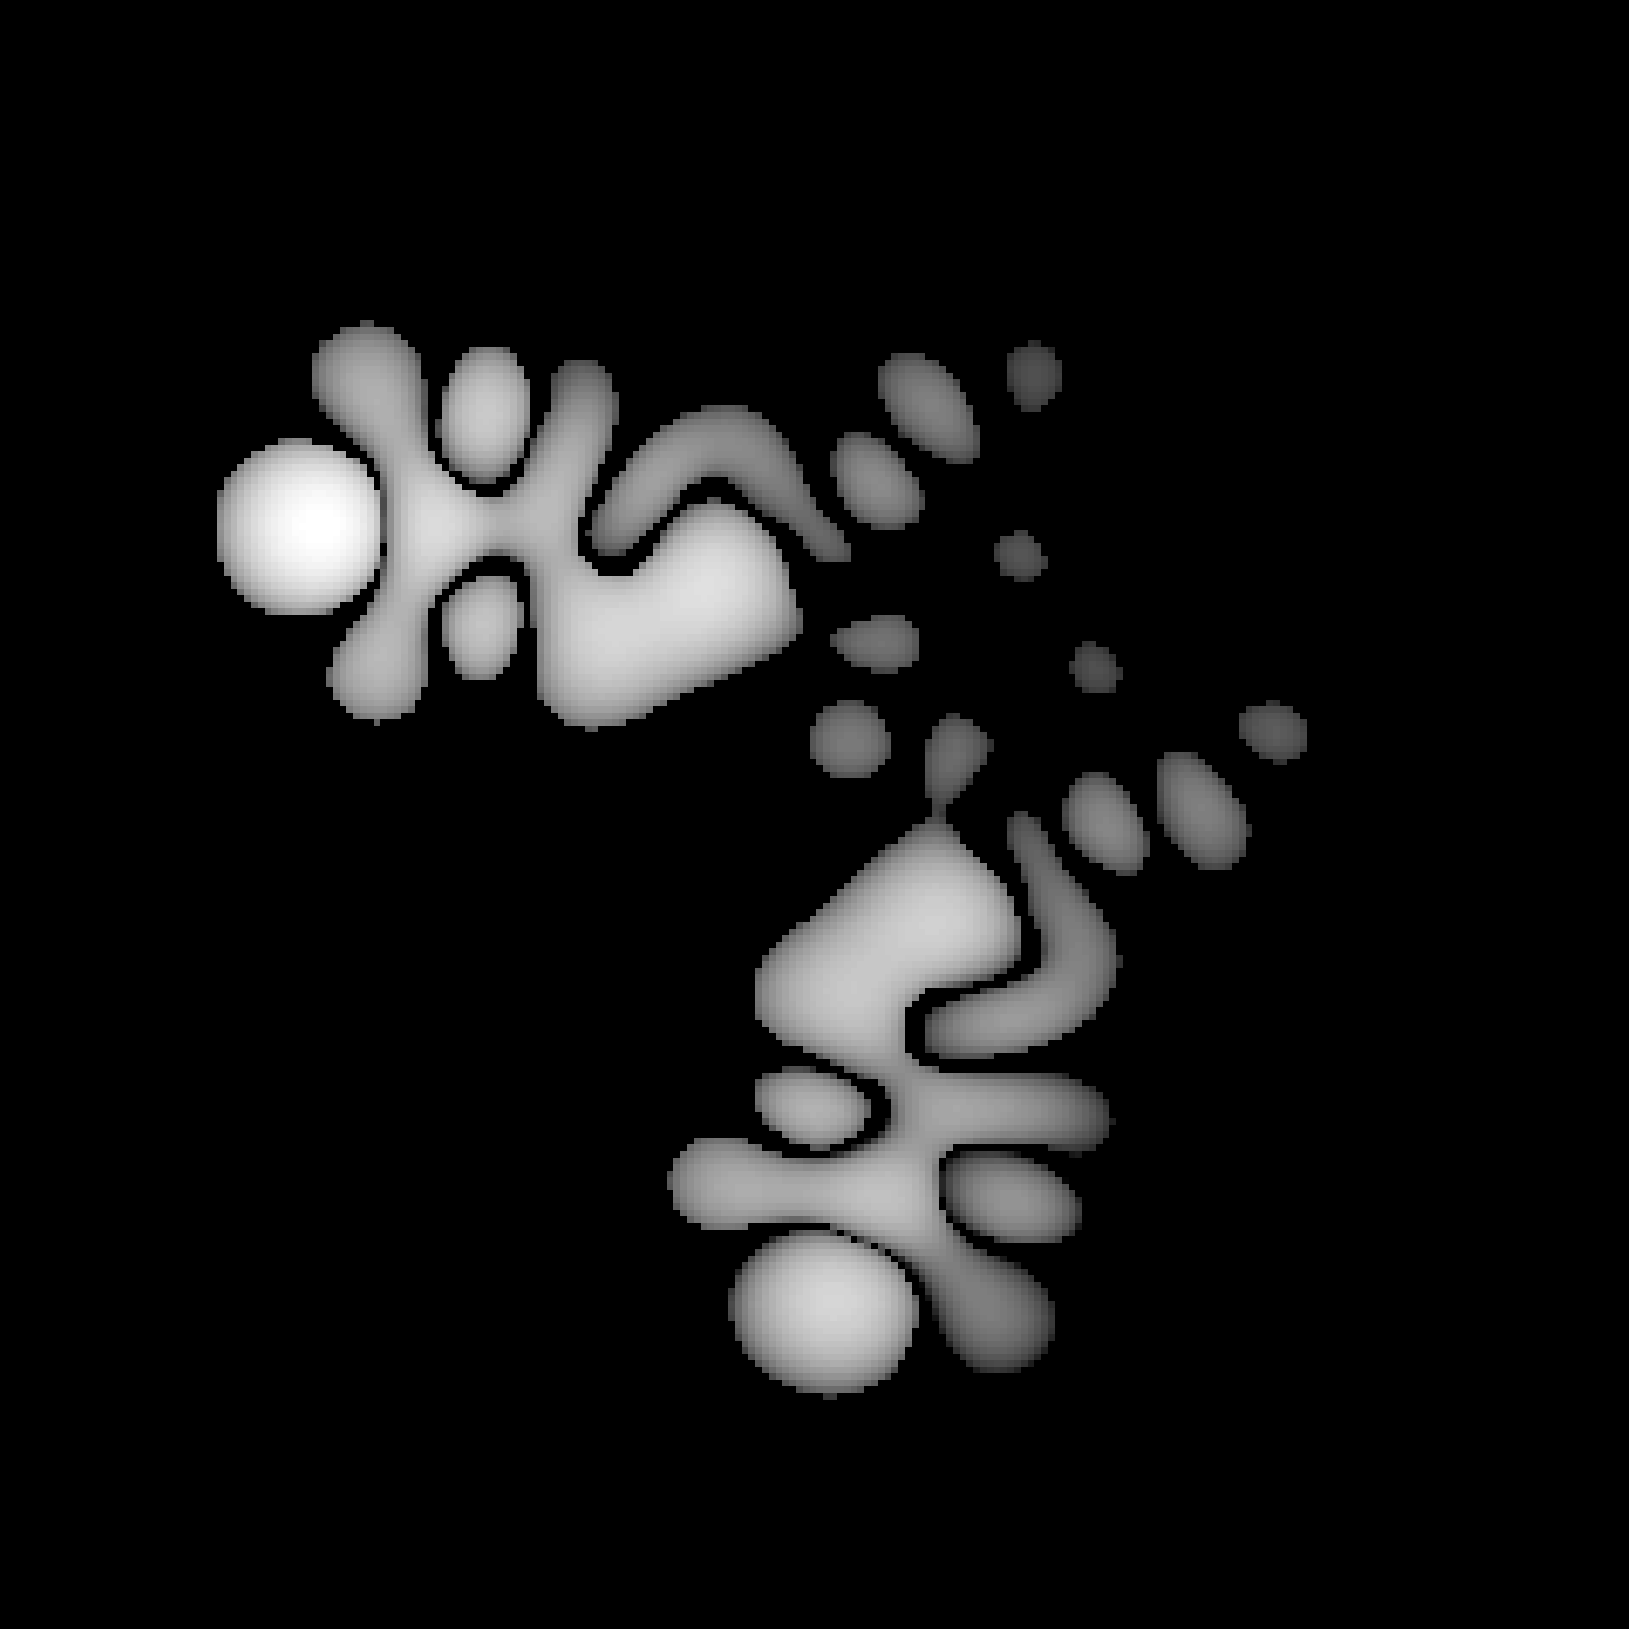
\includegraphics[width=2.7cm]{homo-4}
		\label{fig:homo-4}	
	}
	\subfigure[LUMO + 4]{
		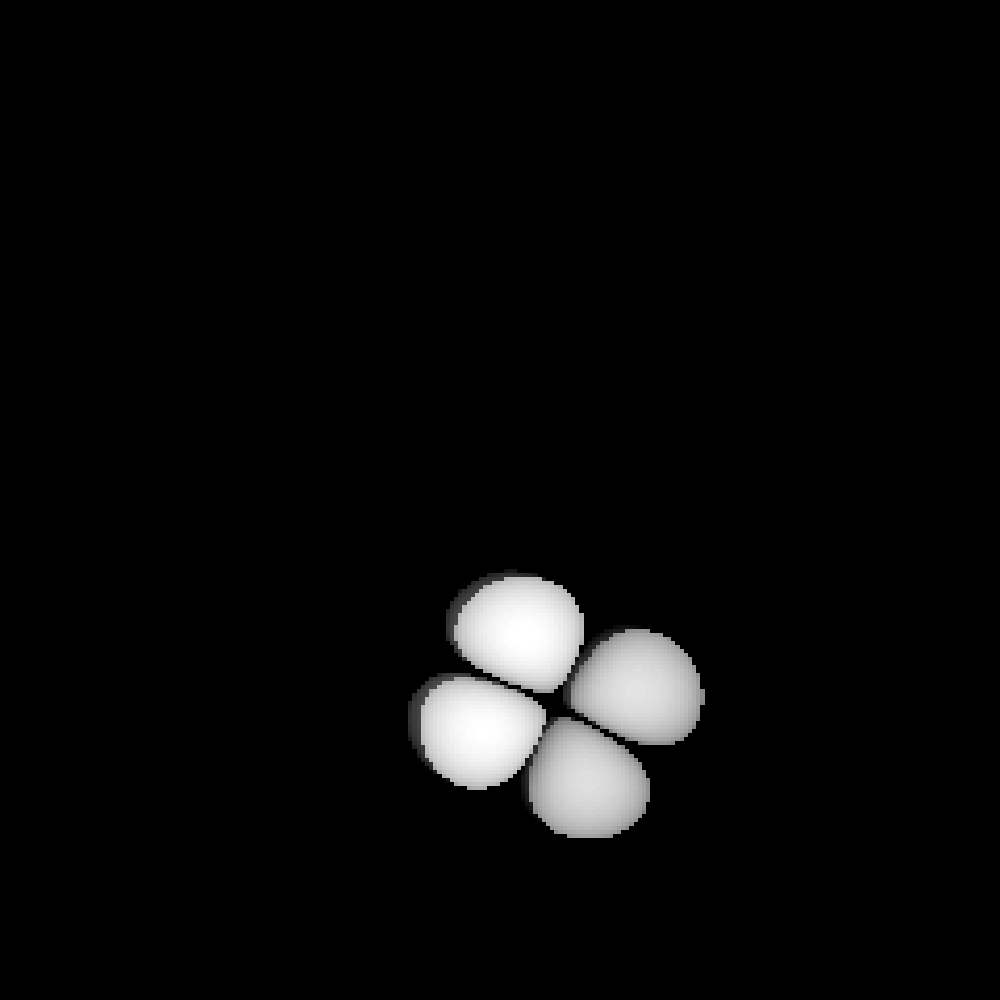
\includegraphics[width=2.7cm]{lumo-4}
		\label{fig:lumo+4}	
	}
	\subfigure[]{
		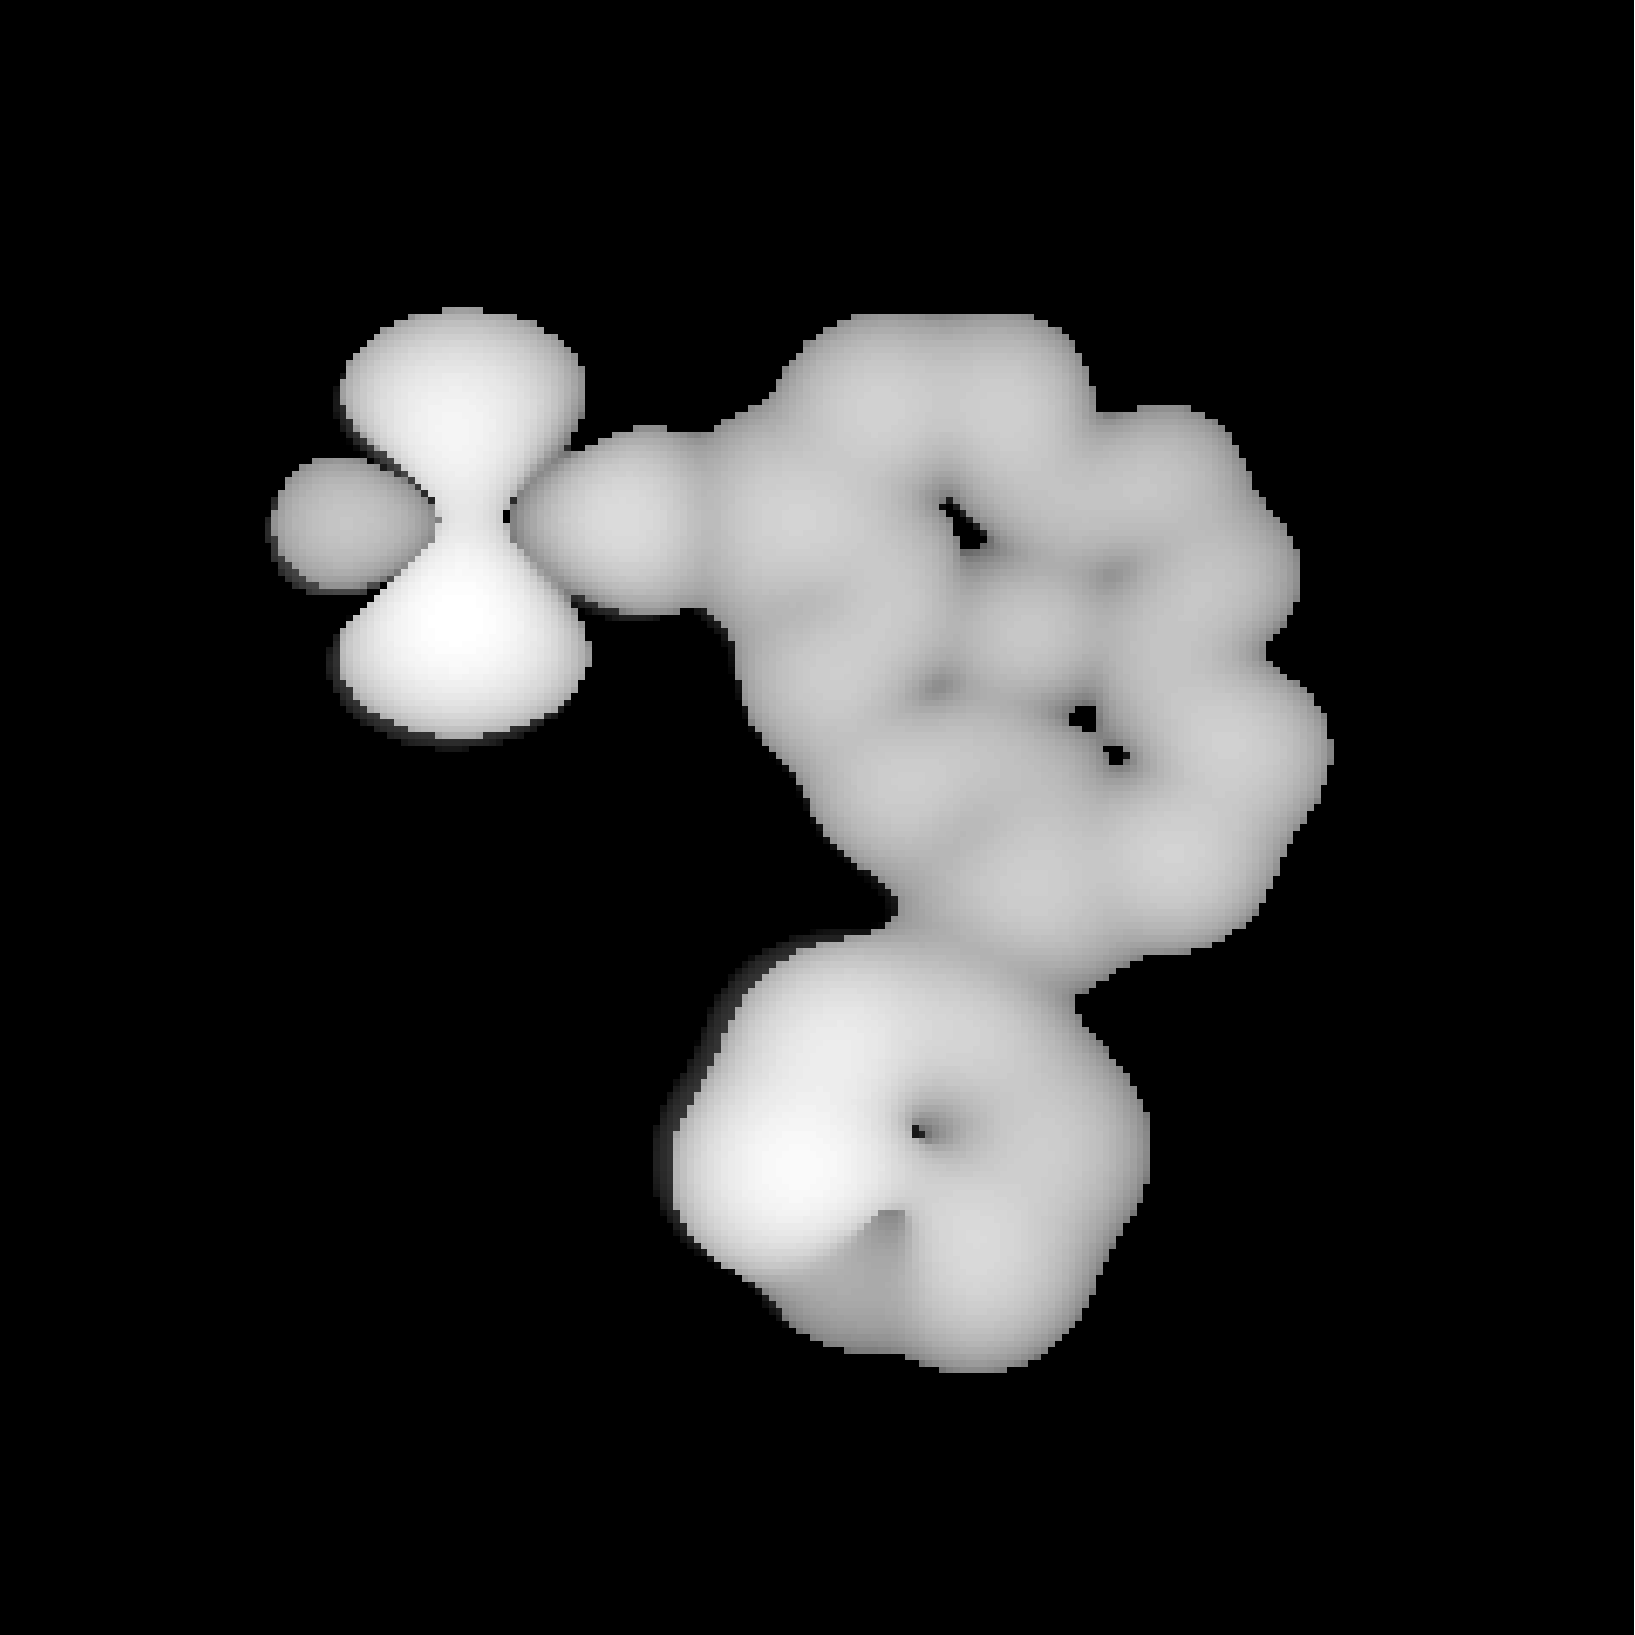
\includegraphics[width=2.7cm]{int-lumo-4}
		\label{fig:}	
	}
	%%%%%%%%%%%%%%%%%%%%%%%%%%%%%%%%%%%%%%%%%
	\subfigure[]{
		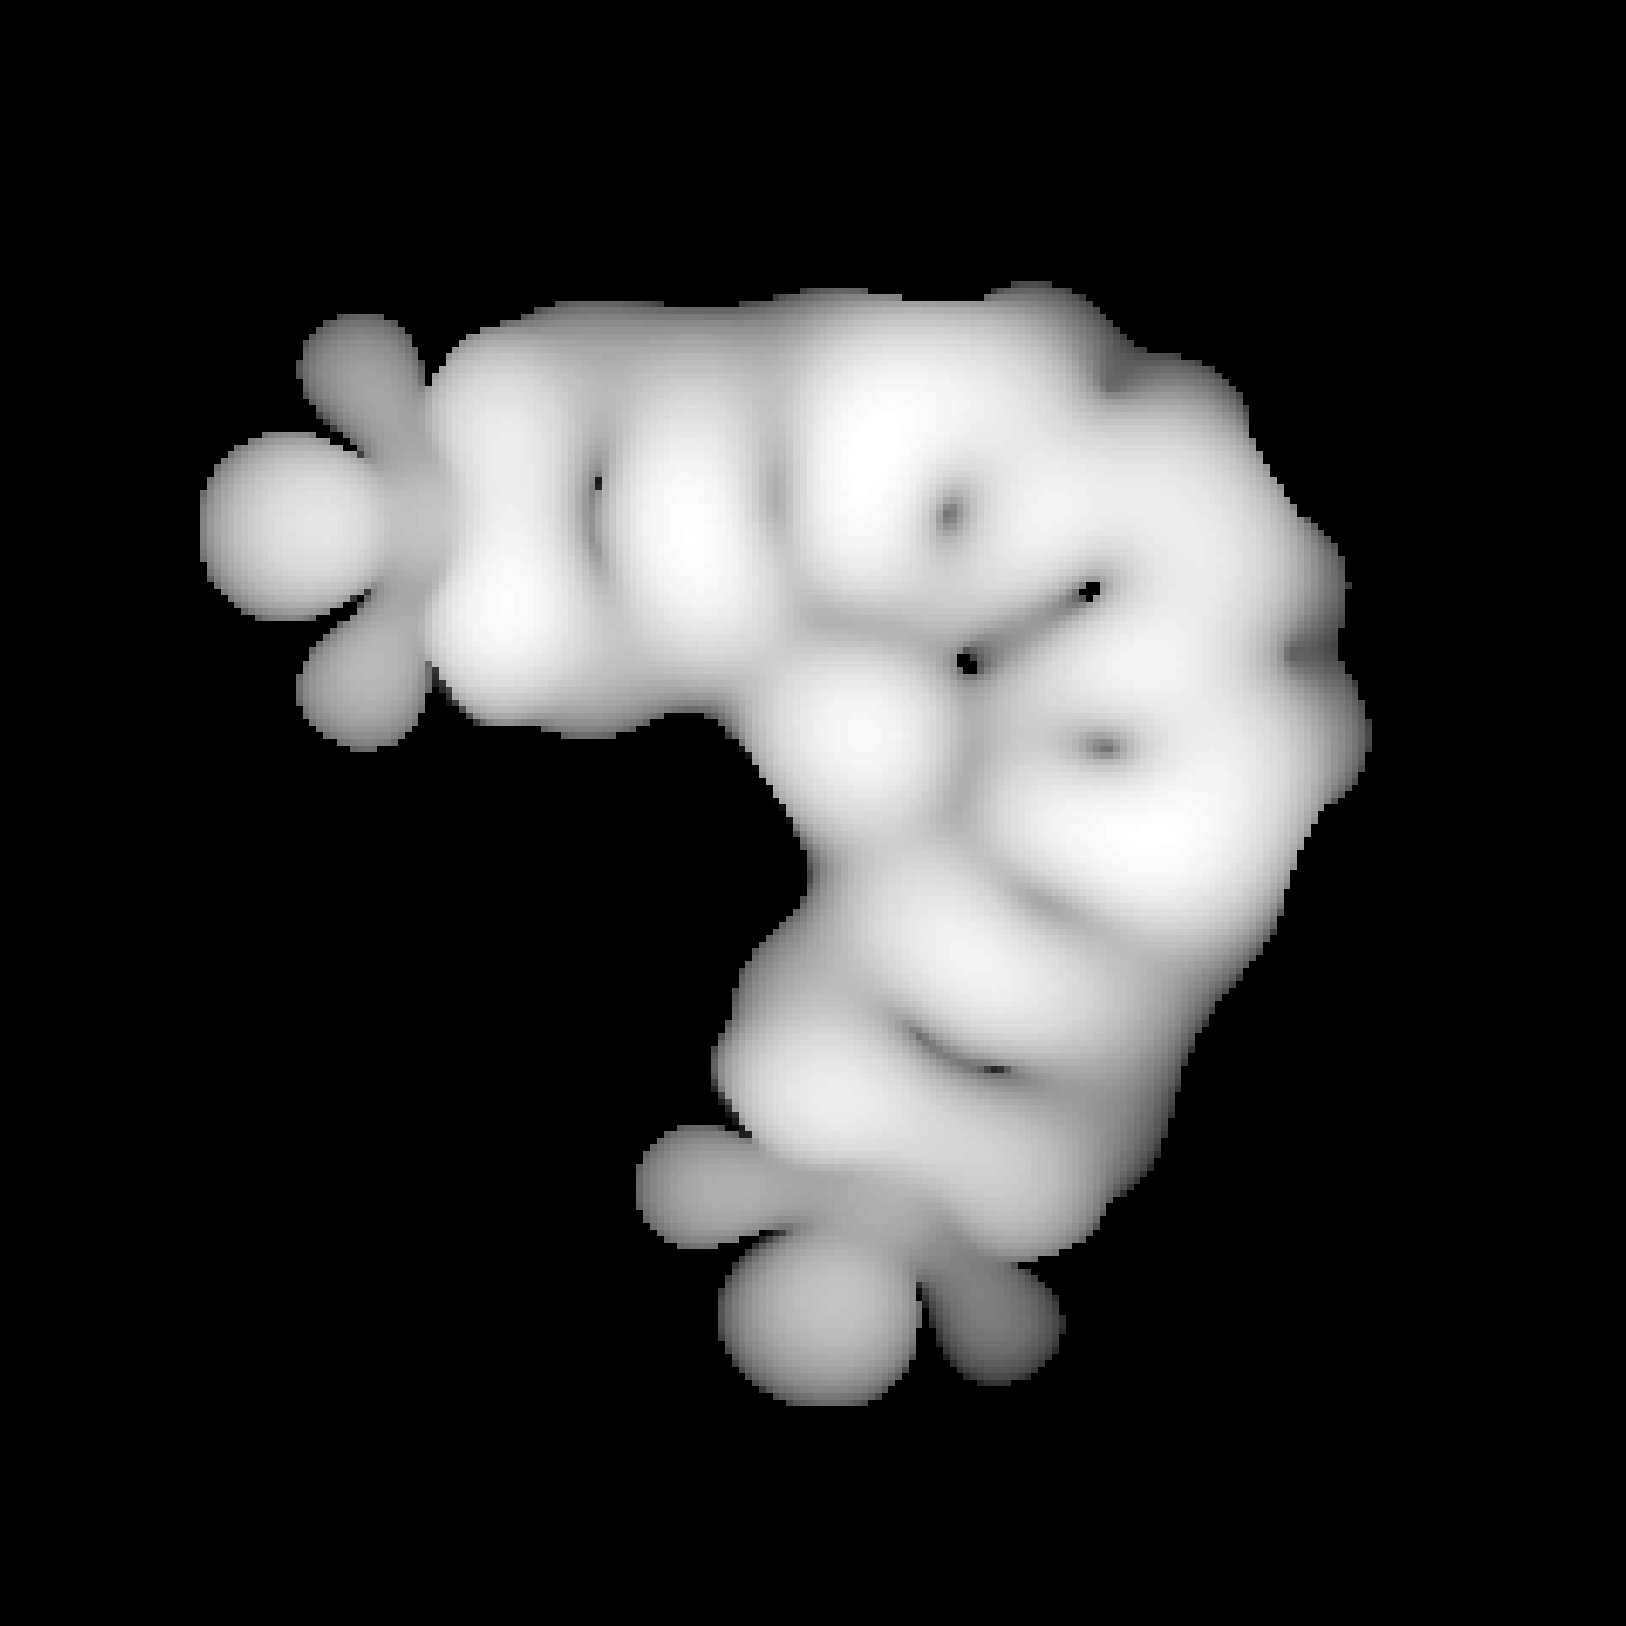
\includegraphics[width=2.7cm]{int-homo-5}
		\label{fig:}
	}
	\subfigure[HOMO - 5]{
		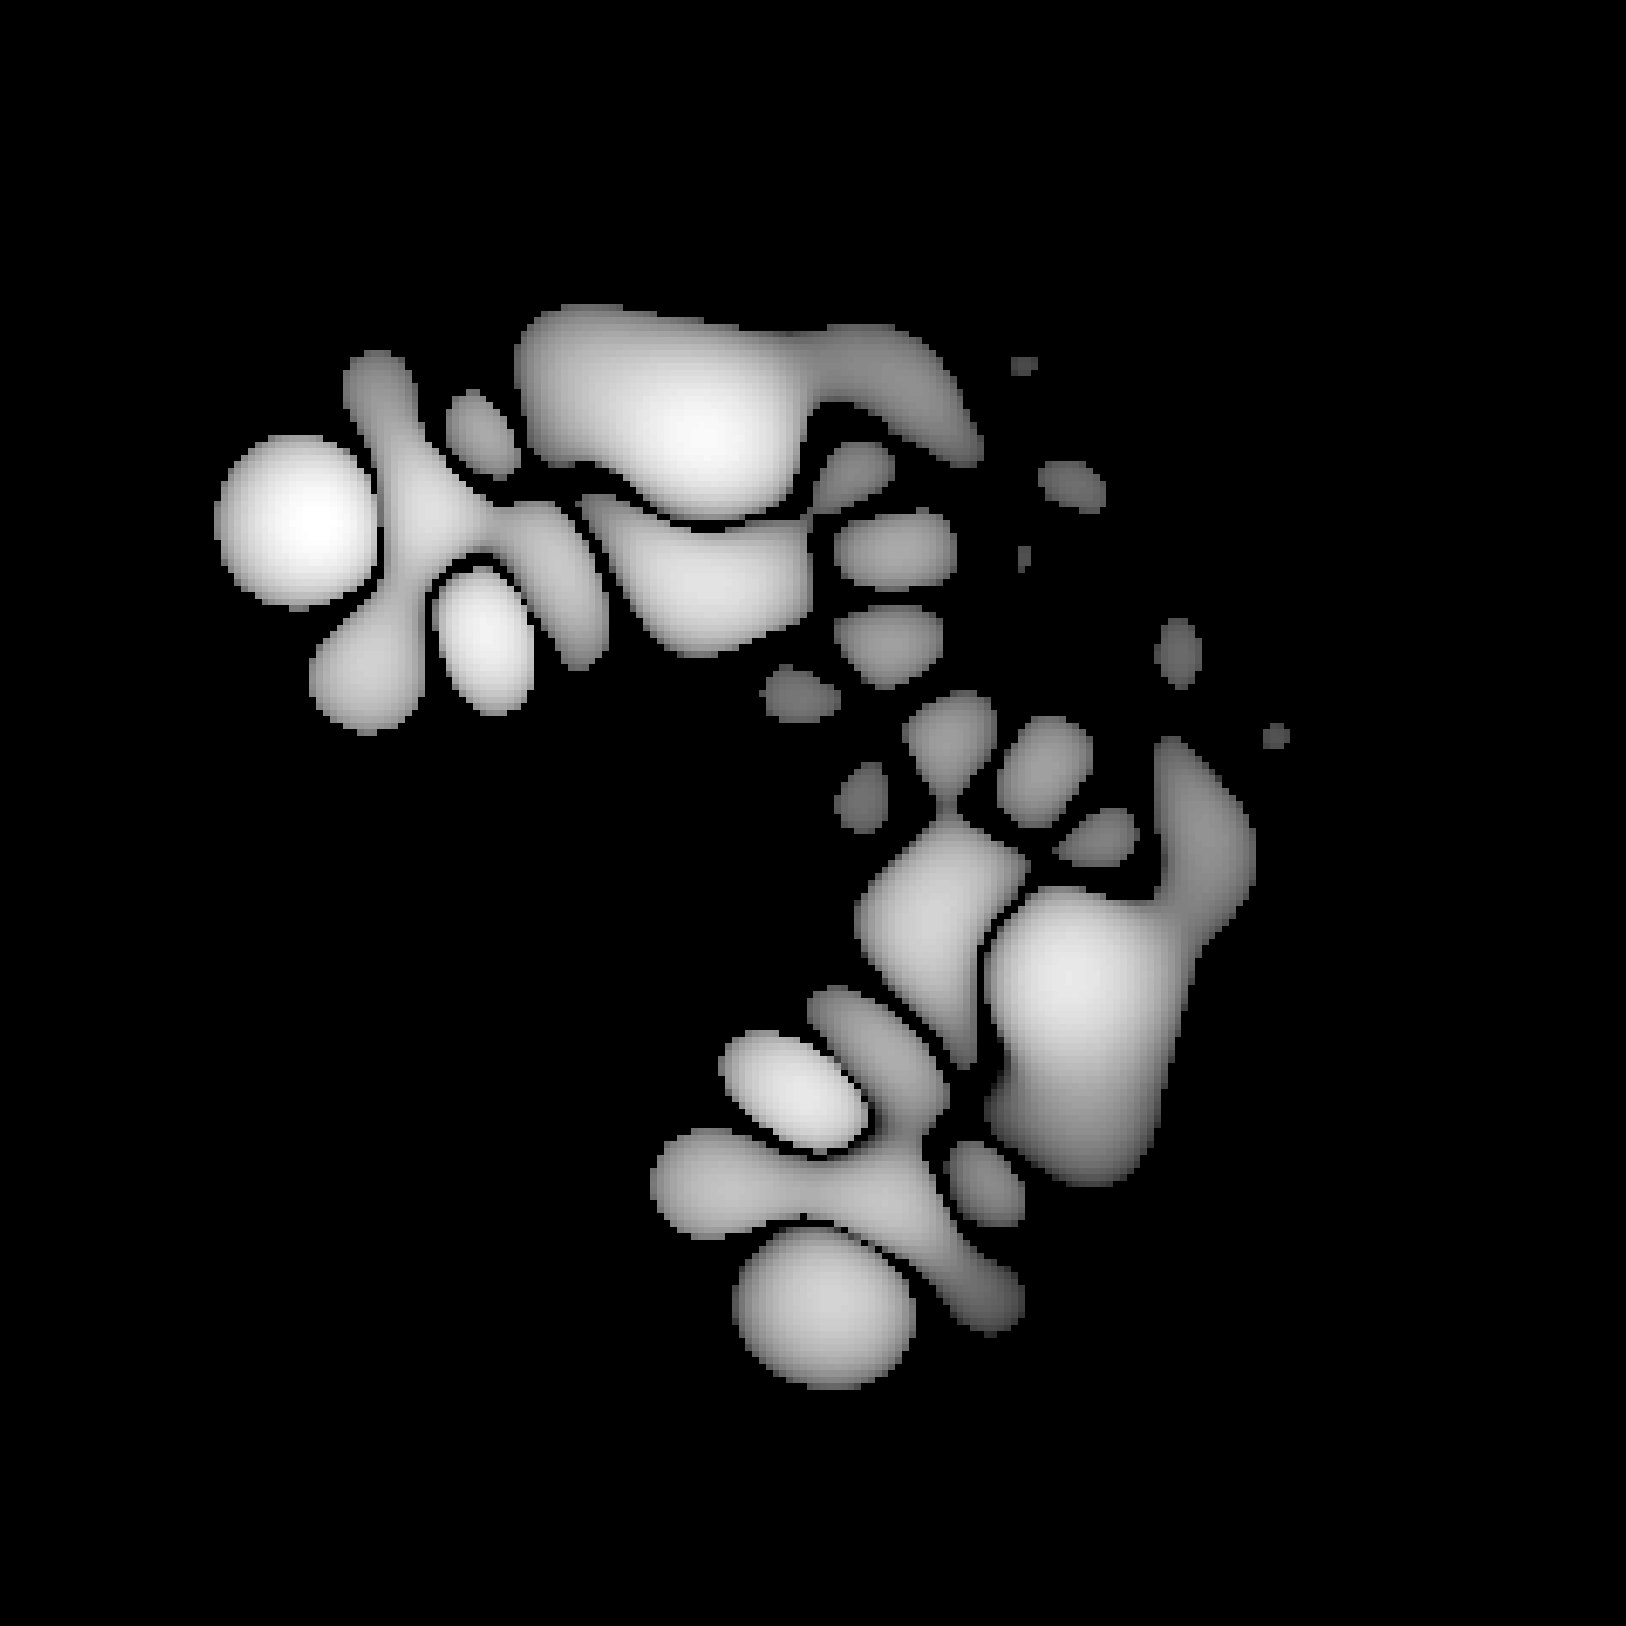
\includegraphics[width=2.7cm]{homo-5}
		\label{fig:homo-5}	
	}
	\subfigure[LUMO + 5]{
		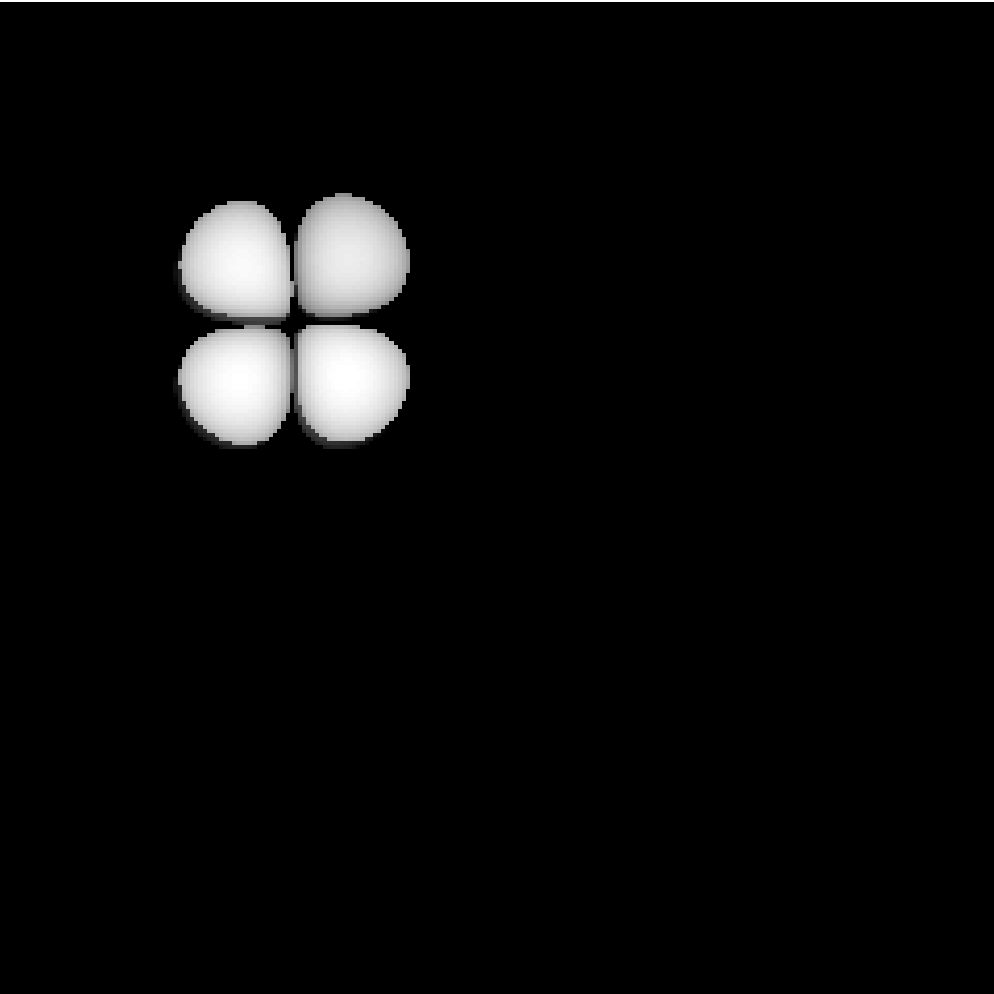
\includegraphics[width=2.7cm]{lumo-5}
		\label{fig:lumo+5}	
	}
	\subfigure[]{
		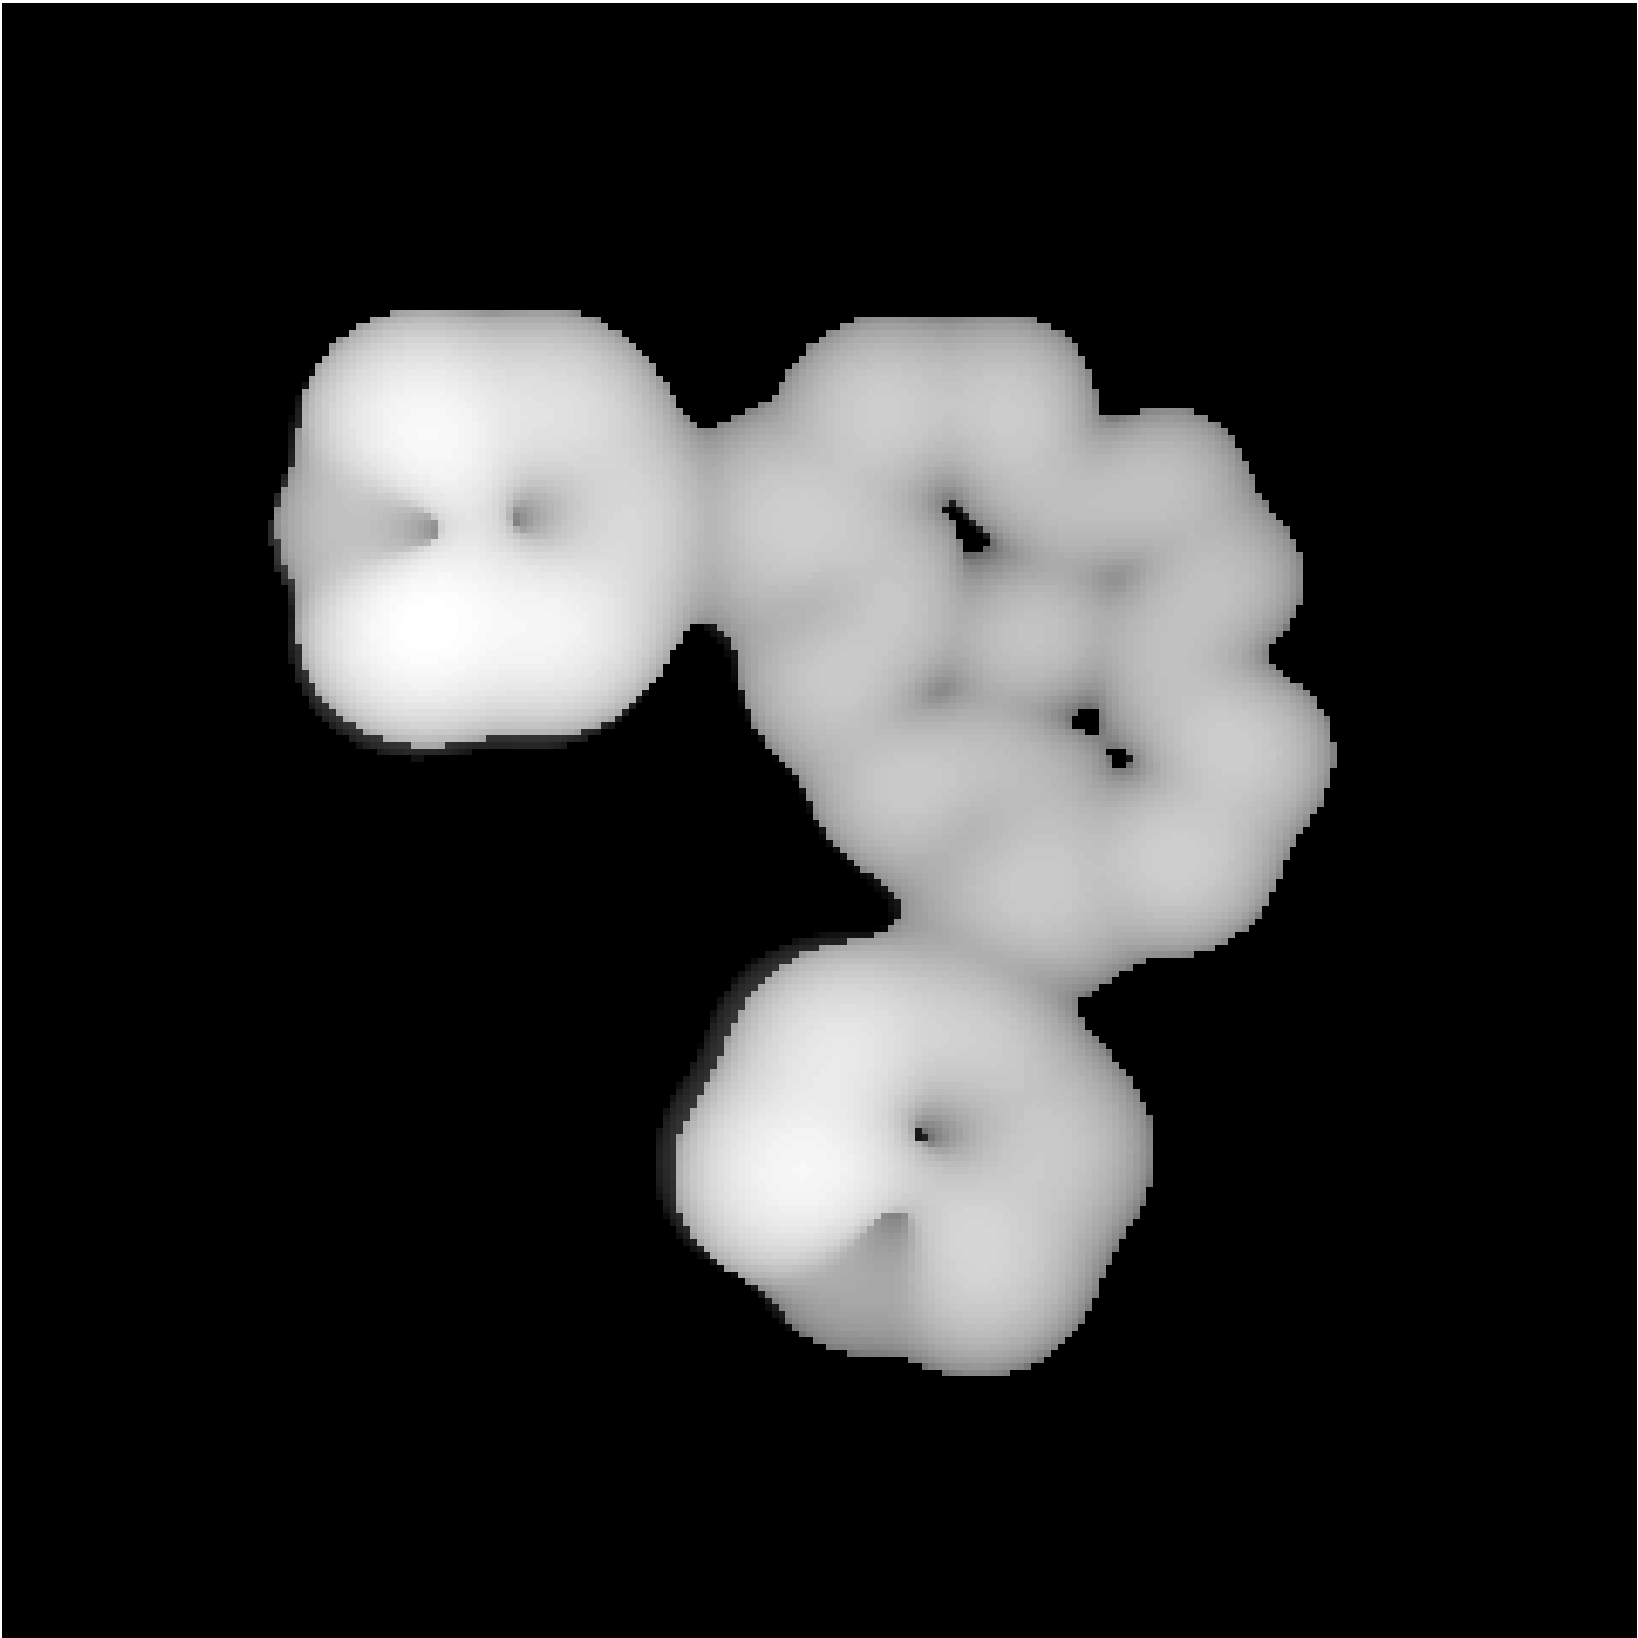
\includegraphics[width=2.7cm]{int-lumo-5}
		\label{fig:}	
	}
	\caption{EHT calculated molecular orbitals. HOMO and LUMO states together with five neighboring states (shown in the same column). Inner two columns show HOMO \& LUMO states. Outer columns show integration of states as STM image estimation if all states to $E_F$ were contributing equally. Images are \SI{2.5}{\nano \meter} wide}
	\label{fig:}
\end{figure}
\vfill